% Lines starting with a percent sign (%) are comments. LaTeX will
% not process those lines. Similarly, everything after a percent
% sign in a line is considered a comment. To produce a percent sign
% in the output, write \% (backslash followed by the percent sign).
% ==================================================================
% Usage instructions:
% ------------------------------------------------------------------
% The file is heavily commented so that you know what the various
% commands do. Feel free to remove any comments you don't need from
% your own copy. When redistributing the example thesis file, please
% retain all the comments for the benefit of other thesis writers!
% ==================================================================
% Compilation instructions:
% ------------------------------------------------------------------
% Use pdflatex to compile! Input images are expected as PDF files.
% Example compilation:
% ------------------------------------------------------------------
% > pdflatex thesis-example.tex
% > bibtex thesis-example
% > pdflatex thesis-example.tex
% > pdflatex thesis-example.tex
% ------------------------------------------------------------------
% You need to run pdflatex multiple times so that all the cross-references
% are fixed. pdflatex will tell you if you need to re-run it (a warning
% will be issued)
% ------------------------------------------------------------------
% Compilation has been tested to work in ukk.cs.hut.fi and kosh.hut.fi
% - if you have problems of missing .sty -files, then the local LaTeX
% environment does not have all the required packages installed.
% For example, when compiling in vipunen.hut.fi, you get an error that
% tikz.sty is missing - in this case you must either compile somewhere
% else, or you cannot use TikZ graphics in your thesis and must therefore
% remove or comment out the tikz package and all the tikz definitions.
% ------------------------------------------------------------------

% General information
% ==================================================================
% Package documentation:
%
% The comments often refer to package documentation. (Almost) all LaTeX
% packages have documentation accompanying them, so you can read the
% package documentation for further information. When a package 'xxx' is
% installed to your local LaTeX environment (the document compiles
% when you have \usepackage{xxx} and LaTeX does not complain), you can
% find the documentation somewhere in the local LaTeX texmf directory
% hierarchy. In ukk.cs.hut.fi, this is /usr/texlive/2008/texmf-dist,
% and the documentation for the titlesec package (for example) can be
% found at /usr/texlive/2008/texmf-dist/doc/latex/titlesec/titlesec.pdf.
% Most often the documentation is located as a PDF file in
% /usr/texlive/2008/texmf-dist/doc/latex/xxx, where xxx is the package name;
% however, documentation for TikZ is in
% /usr/texlive/2008/texmf-dist/doc/latex/generic/pgf/pgfmanual.pdf
% (this is because TikZ is a front-end for PGF, which is meant to be a
% generic portable graphics format for LaTeX).
% You can try to look for the package manual using the ``find'' shell
% command in Linux machines; the find databases are up-to-date at least
% in ukk.cs.hut.fi. Just type ``find xxx'', where xxx is the package
% name, and you should find a documentation file.
% Note that in some packages, the documentation is in the DVI file
% format. In this case, you can copy the DVI file to your home directory,
% and convert it to PDF with the dvipdfm command (or you can read the
% DVI file directly with a DVI viewer).
%
% If you can't find the documentation for a package, just try Googling
% for ``latex packagename''; most often you can get a direct link to the
% package manual in PDF format.
% ------------------------------------------------------------------


% Document class for the thesis is report
% ------------------------------------------------------------------
% You can change this but do so at your own risk - it may break other things.
% Note that the option pdftext is used for pdflatex; there is no
% pdflatex option.
% ------------------------------------------------------------------
\documentclass[12pt,a4paper,oneside,pdftex]{report}

% The input files (tex files) are encoded with the latin-1 encoding
% (ISO-8859-1 works). Change the latin1-option if you use UTF8
% (at some point LaTeX did not work with UTF8, but I'm not sure
% what the current situation is)
\usepackage[utf8]{inputenc}
% OT1 font encoding seems to work better than T1. Check the rendered
% PDF file to see if the fonts are encoded properly as vectors (instead
% of rendered bitmaps). You can do this by zooming very close to any letter
% - if the letter is shown pixelated, you should change this setting
% (try commenting out the entire line, for example).
\usepackage[OT1]{fontenc}
% The babel package provides hyphenating instructions for LaTeX. Give
% the languages you wish to use in your thesis as options to the babel
% package (as shown below). You can remove any language you are not
% going to use.
% Examples of valid language codes: english (or USenglish), british,
% finnish, swedish; and so on.
\usepackage[finnish,swedish,english]{babel}


% Font selection
% ------------------------------------------------------------------
% The default LaTeX font is a very good font for rendering your
% thesis. It is a very professional font, which will always be
% accepted.
% If you, however, wish to spicen up your thesis, you can try out
% these font variants by uncommenting one of the following lines
% (or by finding another font package). The fonts shown here are
% all fonts that you could use in your thesis (not too silly).
% Changing the font causes the layouts to shift a bit; you many
% need to manually adjust some layouts. Check the warning messages
% LaTeX gives you.
% ------------------------------------------------------------------
% To find another font, check out the font catalogue from
% http://www.tug.dk/FontCatalogue/mathfonts.html
% This link points to the list of fonts that support maths, but
% that's a fairly important point for master's theses.
% ------------------------------------------------------------------
% <rant>
% Remember, there is no excuse to use Comic Sans, ever, in any
% situation! (Well, maybe in speech bubbles in comics, but there
% are better options for those too)
% </rant>

%\usepackage{tgcursor}

%\usepackage{nimbus}
%\usepackage[scaled]{helvet}
%\renewcommand*\familydefault{\sfdefault} %% Only if the base font of the document is to be sans serif
% \usepackage{palatino}
% \usepackage{tgpagella}
% \usepackage[bitstream-charter]{mathdesign}

% Optional packages
% ------------------------------------------------------------------
% Select those packages that you need for your thesis. You may delete
% or comment the rest.

% Natbib allows you to select the format of the bibliography references.
% The first example uses numbered citations:
% \usepackage[square,sort&compress,numbers]{natbib}
% The second example uses author-year citations.
% If you use author-year citations, change the bibliography style (below);
% acm style does not work with author-year citations.
% Also, you should use \citet (cite in text) when you wish to refer
% to the author directly (\citet{blaablaa} said blaa blaa), and
% \citep when you wish to refer similarly than with numbered citations
% (It has been said that blaa blaa~\citep{blaablaa}).
\usepackage[round]{natbib}

% The alltt package provides an all-teletype environment that acts
% like verbatim but you can use LaTeX commands in it. Uncomment if
% you want to use this environment.
% \usepackage{alltt}

% The eurosym package provides a euro symbol. Use with \euro{}
\usepackage{eurosym}

% Verbatim provides a standard teletype environment that renderes
% the text exactly as written in the tex file. Useful for code
% snippets (although you can also use the listings package to get
% automatic code formatting).
\usepackage{verbatim}

% The listing package provides automatic code formatting utilities
% so that you can copy-paste code examples and have them rendered
% nicely. See the package documentation for details.
% \usepackage{listings}

% The fancuvrb package provides fancier verbatim environments
% (you can, for example, put borders around the verbatim text area
% and so on). See package for details.
% \usepackage{fancyvrb}

% Supertabular provides a tabular environment that can span multiple
% pages.
%\usepackage{supertabular}
% Longtable provides a tabular environment that can span multiple
% pages. This is used in the example acronyms file.
\usepackage{longtable}

% The fancyhdr package allows you to set your the page headers
% manually, and allows you to add separator lines and so on.
% Check the package documentation.
% \usepackage{fancyhdr}

% Subfigure package allows you to use subfigures (i.e. many subfigures
% within one figure environment). These can have different labels and
% they are numbered automatically. Check the package documentation.
\usepackage{subfigure}

% The titlesec package can be used to alter the look of the titles
% of sections, chapters, and so on. This example uses the ``medium''
% package option which sets the titles to a medium size, making them
% a bit smaller than what is the default. You can fine-tune the
% title fonts and sizes by using the package options. See the package
% documentation.
\usepackage[medium]{titlesec}

% The TikZ package allows you to create professional technical figures.
% The learning curve is quite steep, but it is definitely worth it if
% you wish to have really good-looking technical figures.
\usepackage{tikz}
% You also need to specify which TikZ libraries you use

\usepackage{changepage}
\usetikzlibrary{positioning}
\usetikzlibrary{calc}
\usetikzlibrary{arrows}
\usetikzlibrary{decorations.pathmorphing,decorations.markings}
\usetikzlibrary{shapes}
\usetikzlibrary{patterns}
\usetikzlibrary{chains}

% The aalto-thesis package provides typesetting instructions for the
% standard master's thesis parts (abstracts, front page, and so on)
% Load this package second-to-last, just before the hyperref package.
% Options that you can use:
%   mydraft - renders the thesis in draft mode.
%             Do not use for the final version.
%   doublenumbering - [optional] number the first pages of the thesis
%                     with roman numerals (i, ii, iii, ...); and start
%                     arabic numbering (1, 2, 3, ...) only on the
%                     first page of the first chapter
%   twoinstructors  - changes the title of instructors to plural form
%   twosupervisors  - changes the title of supervisors to plural form
\usepackage[mydraft,twosupervisors]{aalto-thesis}
%\usepackage[mydraft,doublenumbering]{aalto-thesis}
%\usepackage{aalto-thesis}


% Hyperref
% ------------------------------------------------------------------
% Hyperref creates links from URLs, for references, and creates a
% TOC in the PDF file.
% This package must be the last one you include, because it has
% compatibility issues with many other packages and it fixes
% those issues when it is loaded.
\RequirePackage[pdftex]{hyperref}
% Setup hyperref so that links are clickable but do not look
% different
\hypersetup{colorlinks=false,raiselinks=false,breaklinks=true}
\hypersetup{pdfborder={0 0 0}}
\hypersetup{bookmarksnumbered=true}
% The following line suggests the PDF reader that it should show the
% first level of bookmarks opened in the hierarchical bookmark view.
\hypersetup{bookmarksopen=true,bookmarksopenlevel=1}
% Hyperref can also set up the PDF metadata fields. These are
% set a bit later on, after the thesis setup.


% Thesis setup
% ==================================================================
% Change these to fit your own thesis.
% \COMMAND always refers to the English version;
% \FCOMMAND refers to the Finnish version; and
% \SCOMMAND refers to the Swedish version.
% You may comment/remove those language variants that you do not use
% (but then you must not include the abstracts for that language)
% ------------------------------------------------------------------
% If you do not find the command for a text that is shown in the cover page or
% in the abstract texts, check the aalto-thesis.sty file and locate the text
% from there.
% All the texts are configured in language-specific blocks (lots of commands
% that look like this: \renewcommand{\ATCITY}{Espoo}.
% You can just fix the texts there. Just remember to check all the language
% variants you use (they are all there in the same place).
% ------------------------------------------------------------------
\newcommand{\TITLE}{Developing a framework for software integration through continuous testing}
\newcommand{\FTITLE}{TODO}
\newcommand{\STITLE}{TODO}
\newcommand{\SUBTITLE}{Case Wärtsilä}
\newcommand{\FSUBTITLE}{TODO}
\newcommand{\SSUBTITLE}{TODO}
\newcommand{\DATE}{January 18, 2013}
\newcommand{\FDATE}{18. tammikuuta 2013}
\newcommand{\SDATE}{Den 18 Januari 2013}

% Supervisors and instructors
% ------------------------------------------------------------------
% If you have two supervisors, write both names here, separate them with a
% double-backslash (see below for an example)
% Also remember to add the package option ``twosupervisors'' or
% ``twoinstructors'' to the aalto-thesis package so that the titles are in
% plural.
% Example of one supervisor:
%\newcommand{\SUPERVISOR}{Professor Antti Ylä-Jääski}
%\newcommand{\FSUPERVISOR}{Professori Antti Ylä-Jääski}
%\newcommand{\SSUPERVISOR}{Professor Antti Ylä-Jääski}
% Example of twosupervisors:
\newcommand{\SUPERVISOR}{Professor Riitta Smeds}
\newcommand{\FSUPERVISOR}{Professor Riitta Smeds}
\newcommand{\SSUPERVISOR}{Professor Riitta Smeds}

% If you have only one instructor, just write one name here
\newcommand{\INSTRUCTOR}{Eero Tuomikoski M.Sc. (Tech.)}
\newcommand{\FINSTRUCTOR}{Diplomi-insinööri Eero Tuomikoski}
\newcommand{\SINSTRUCTOR}{Diplomingenjör Eero Tuomikoski}
% If you have two instructors, separate them with \\ to create linefeeds
% \newcommand{\INSTRUCTOR}{Olli Ohjaaja M.Sc. (Tech.)\\
%  Elli Opas M.Sc. (Tech)}
%\newcommand{\FINSTRUCTOR}{Diplomi-insinööri Olli Ohjaaja\\
%  Diplomi-insinööri Elli Opas}
%\newcommand{\SINSTRUCTOR}{Diplomingenjör Olli Ohjaaja\\
%  Diplomingenjör Elli Opas}

% If you have two supervisors, it is common to write the schools
% of the supervisors in the cover page. If the following command is defined,
% then the supervisor names shown here are printed in the cover page. Otherwise,
% the supervisor names defined above are used.
\newcommand{\COVERSUPERVISOR}{Professor Riitta Smeds, Aalto University}

% The same option is for the instructors, if you have multiple instructors.
% \newcommand{\COVERINSTRUCTOR}{Olli Ohjaaja M.Sc. (Tech.), Aalto University\\
%  Elli Opas M.Sc. (Tech), Aalto SCI}


% Other stuff
% ------------------------------------------------------------------
\newcommand{\PROFESSORSHIP}{Data Communication Software}
\newcommand{\FPROFESSORSHIP}{Tietoliikenneohjelmistot}
\newcommand{\SPROFESSORSHIP}{Datakommunikationsprogram}
% Professorship code is the same in all languages
\newcommand{\PROFCODE}{T-110}
\newcommand{\KEYWORDS}{integration testing, testing automation, testing frameworks}
\newcommand{\FKEYWORDS}{ohjelmistotestaus, automatisoitu testaus, integraatiotestaus}
\newcommand{\SKEYWORDS}{testning}
\newcommand{\LANGUAGE}{English}
\newcommand{\FLANGUAGE}{Englanti}
\newcommand{\SLANGUAGE}{Engelska}

% Author is the same for all languages
\newcommand{\AUTHOR}{Antti Heikkonen}


% Currently the English versions are used for the PDF file metadata
% Set the PDF title
\hypersetup{pdftitle={\TITLE\ \SUBTITLE}}
% Set the PDF author
\hypersetup{pdfauthor={\AUTHOR}}
% Set the PDF keywords
\hypersetup{pdfkeywords={\KEYWORDS}}
% Set the PDF subject
\hypersetup{pdfsubject={Master's Thesis}}


% Layout settings
% ------------------------------------------------------------------

% When you write in English, you should use the standard LaTeX
% paragraph formatting: paragraphs are indented, and there is no
% space between paragraphs.
% When writing in Finnish, we often use no indentation in the
% beginning of the paragraph, and there is some space between the
% paragraphs.

% If you write your thesis Finnish, uncomment these lines; if
% you write in English, leave these lines commented!
% \setlength{\parindent}{0pt}
% \setlength{\parskip}{1ex}

% Use this to control how much space there is between each line of text.
% 1 is normal (no extra space), 1.3 is about one-half more space, and
% 1.6 is about double line spacing.
% \linespread{1} % This is the default
% \linespread{1.3}

% Bibliography style
% acm style gives you a basic reference style. It works only with numbered
% references.
% \bibliographystyle{acm}
% Plainnat is a plain style that works with both numbered and name citations.
\bibliographystyle{kbib}


% Extra hyphenation settings
% ------------------------------------------------------------------
% You can list here all the files that are not hyphenated correctly.
% You can provide many \hyphenation commands and/or separate each word
% with a space inside a single command. Put hyphens in the places where
% a word can be hyphenated.
% Note that (by default) LaTeX will not hyphenate words that already
% have a hyphen in them (for example, if you write ``structure-modification
% operation'', the word structure-modification will never be hyphenated).
% You need a special package to hyphenate those words.
\hyphenation{di-gi-taa-li-sta yksi-suun-tai-sta}



% The preamble ends here, and the document begins.
% Place all formatting commands and such before this line.
% ------------------------------------------------------------------
\begin{document}
% This command adds a PDF bookmark to the cover page. You may leave
% it out if you don't like it...
\pdfbookmark[0]{Cover page}{bookmark.0.cover}
% This command is defined in aalto-thesis.sty. It controls the page
% numbering based on whether the doublenumbering option is specified
\startcoverpage

% Cover page
% ------------------------------------------------------------------
% Options: finnish, english, and swedish
% These control in which language the cover-page information is shown
\coverpage{english}


% Abstracts
% ------------------------------------------------------------------
% Include an abstract in the language that the thesis is written in,
% and if your native language is Finnish or Swedish, one in that language.

% Abstract in English
% ------------------------------------------------------------------
\thesisabstract{english}{
A dissertation or thesis is a document submitted in support of candidature
for a degree or professional qualification presenting the author's research and
findings. In some countries/universities, the word thesis or a cognate is used
as part of a bachelor's or master's course, while dissertation is normally
applied to a doctorate, whilst, in others, the reverse is true.

\fixme{Abstract text goes here (and this is an example how to use fixme).}
Fixme is a command that helps you identify parts of your thesis that still
require some work. When compiled in the custom \texttt{mydraft} mode, text
parts tagged with fixmes are shown in bold and with fixme tags around them. When
compiled in normal mode, the fixme-tagged text is shown normally (without
special formatting). The draft mode also causes the ``Draft'' text to appear on
the front page, alongside with the document compilation date. The custom
\texttt{mydraft} mode is selected by the \texttt{mydraft} option given for the
package \texttt{aalto-thesis}, near the top of the \texttt{thesis-example.tex}
file.

The thesis example file (\texttt{thesis-example.tex}), all the chapter content
files (\texttt{1introduction.tex} and so on), and the Aalto style file
(\texttt{aalto-thesis.sty}) are commented with explanations on how the Aalto
thesis works. The files also contain some examples on how to customize various
details of the thesis layout, and of course the example text works as an
example in itself. Please read the comments and the example text; that should
get you well on your way!}

% Abstract in Finnish
% ------------------------------------------------------------------
\thesisabstract{finnish}{
Tiivistelmä}

% Abstract in Swedish
% ------------------------------------------------------------------
\thesisabstract{swedish}{
Referat.}


% Acknowledgements
% ------------------------------------------------------------------
% Select the language you use in your acknowledgements
\selectlanguage{english}

% Uncomment this line if you wish acknoledgements to appear in the
% table of contents
%\addcontentsline{toc}{chapter}{Acknowledgements}

% The star means that the chapter isn't numbered and does not
% show up in the TOC
\chapter*{Acknowledgements}

I wish to thank all students who use \LaTeX\ for formatting their theses,
because theses formatted with \LaTeX\ are just so nice.

Thank you, and keep up the good work!
\vskip 10mm

\noindent Helsinki, \DATE
\vskip 5mm
\noindent\AUTHOR

% Acronyms
% ------------------------------------------------------------------
% Use \cleardoublepage so that IF two-sided printing is used
% (which is not often for masters theses), then the pages will still
% start correctly on the right-hand side.
\cleardoublepage
% Example acronyms are placed in a separate file, acronyms.tex
% \input{acronyms}

\addcontentsline{toc}{chapter}{Abbreviations and Acronyms}
\chapter*{Abbreviations and Acronyms}

% The longtable environment should break the table properly to multiple pages,
% if needed

\noindent
\begin{longtable}{@{}p{0.25\textwidth}p{0.7\textwidth}@{}}
SOA & Service-oritented architecture \\
UTF & Unified testing framework \\
WSDL & Web service description language \\
WTF & Wärtsilä testing framework \\
% e.g.& for example (do not list here this kind of common acronymbs or abbreviations, but only those that are essential for understanding the content of your thesis. \\
% note & Note also, that this list is not compulsory, and should be omitted if you have only few abbreviations

\end{longtable}


% Table of contents
% ------------------------------------------------------------------
\cleardoublepage
% This command adds a PDF bookmark that links to the contents.
% You can use \addcontentsline{} as well, but that also adds contents
% entry to the table of contents, which is kind of redundant.
% The text ``Contents'' is shown in the PDF bookmark.
\pdfbookmark[0]{Contents}{bookmark.0.contents}
\tableofcontents

% List of tables
% ------------------------------------------------------------------
% You only need a list of tables for your thesis if you have very
% many tables. If you do, uncomment the following two lines.
% \cleardoublepage
% \listoftables

% Table of figures
% ------------------------------------------------------------------
% You only need a list of figures for your thesis if you have very
% many figures. If you do, uncomment the following two lines.
% \cleardoublepage
% \listoffigures

% The following label is used for counting the prelude pages
\label{pages-prelude}
\cleardoublepage

%%%%%%%%%%%%%%%%% The main content starts here %%%%%%%%%%%%%%%%%%%%%
% ------------------------------------------------------------------
% This command is defined in aalto-thesis.sty. It controls the page
% numbering based on whether the doublenumbering option is specified
\startfirstchapter

% Add headings to pages (the chapter title is shown)
\pagestyle{headings}

% The contents of the thesis are separated to their own files.
% Edit the content in these files, rename them as necessary.
% ------------------------------------------------------------------

% \input{1introduction.tex}
\chapter{Introduction}
\label{chapter:intro}
% Keywords: system-to-system integration (testing), automated testing, testing framework, integration testing

% benefits of automation, build-up to integration, orienting to automoated IT business processes
% TODO start with key concept, not automation, real-time processes perspective, inter-company, information flow as a % reaso, add picture and figure, why was the work conducted? business critical and dependencies. why?
Automation is one of the great boons brought on by technological development on one hand freeing up resources like labour for more value-adding purposes --- and permitting the execution of uniform, repeatable processes and process control on the other. The pinnacle of advancement and prosperity on which society stands today is based on a continuous flow of various automated tasks and electronic services, many of which are complex and involve a slew of actors or agents. Work is divided and its completion therefore requires cooperation between service systems, which poses another challenge.

% integration reasons and logic
Integrating disparate actors and information systems is a prerequisite of automation. The principles and drivers of  a distributed system are not unlike those behind the division of labour. Complex tasks are easier to solve when divided and each part administered by a dedicated expert. Distributed systems also enable incremental growth, which, of course, is sometimes a less-consciously-pursued natural evolution and accretion of new information services. Other benefits of an interdependent and connected information technology system include a reduction in the number of systems related upkeep, maintenance, and development costs, which also reduces the degree of complexity in the set-up. Shared resources bring economies of scale.

% The negatives in integrated systems.  
Integration efforts may, however, result in unclear responsibilities and difficulties in determining if the systems cooperate and behave correctly, and if any use cases are unaccounted for. In a distributed system there are more components and connections that can fail, and relinquishing control over units always carries risk. A high number of integrations makes the task even more difficult since a single change in the system components can disrupt a whole chain of operation.

% business motivation and technical considerations 
The benefits outweighing all shortcomings, modern coprorations' business processes rely on automation and operate on distributed systems and networked devices. But the problems are still there; ensuring quality of service is essential. Systematic, rigorous, and automated testing, both functional and non-functional, is required. This thesis examines the requirements of system-to-system integration testing in a real world business setting. The hypothesis is that a setup will help uncover defects and issues earlier and resolve them with fewer resources.

\section{Research question}

The overall research problem is to devise a testing framework for automated integration tests. Here, framework refers to both the testing solution technology and libraries. Quality measures, which include functional and non-functional aspects, are described in more detail in chapter X. % TODO chapter num

The research problem can be divided into three questions: \\

% 1. Determine requirements.
\begin{adjustwidth}{2.5em}{0pt}
\textbf{1. What are the requirements for a testing framework in the context of the W{\"a}rtsil{\"a} integration set-up and how should the framework be structured?} \\
\\
% lifecycle, interoperability (change underlying platform), maintenance, licence, architectural fit
The first part addresses the pertinent question: what is a framework? Based on academic literature, a testing framework is modeled and described, which serves as a foundation for answering the second research question. Included in answering the first research question is requirements analysis, i.e. criteria for a suitable framework structure. The requirements are based on W{\"a}rtsil{\"a}'s IT operation environment. .This includes canonical examples of electronic business processes and integrations, for instance between the ERP system and warehouse systems, and the ERP system and the PDM system \\
\\
% 2. Compare alternatives, choose best one.
\textbf{2. Which is the best integration testing framework in of the requirements among a limited set of alternatives?} \\
\\
Promising framework alternatives are listed after which, based on the requirements, a shortlist is composed. The purpose is not to go arduously through every available tool and painstakingly analyze and quantify their potential, but by quick assessment determine a set of alternatives that are easy to use and fit the framework, then offer a succinct comparison. Included in the second research question is requirements analysis, i.e. criteria for suitable framework technologies. A group of selected technologies satisfying the defined framework requirements will constitute a proof of concept experiement. \\
\\
% 3. Test viability. Proof of concept.
\textbf{3. How can the selected framework be implemented?} \\
\\
Answering the third research question involves proofing the selected frameworks. This is a smoke test of the suitability of the chosen framework, but the actual implementation of the test framework and adopting is not part of the thesis. The third research question also includes evaluation \emph{how} the end solution meets previously defined criteria. Any other issues and concerns that arise during the third part are also discussed. \\
\end{adjustwidth}

Additionally, observed results and conclusions are used to produce a set of guidelines and recommendations listed in a separate document (see attachment x). % TODO attachment num

% TODO: consult professor, instructor about research method. Alternatives: exploratory research, empirical research
\section{Research methods}
Research is conducted according to the constructive research method paradigm --- a six step model, where a concrete, real world problem is investigated through practical experience and academic understanding. The resulting conclusions and concepts are then tested in a working simulation. The emphasis is not to produce hard fact to the academic canon, but to produce hypotheses and theories, and test them in practice.
% TODO: insert citations and chart depecting research method

As a scientific work, and to satisfy the first two steps, the thesis's research problem must be relevant enough to be interesting, and robust enough for academic research. The third crucial step entails the construction of a novel solution and new understanding, which are then argued in step four with the purpose of demonstrating that the built construct works. In the fifth step the researcher compares the solution to theoretical models and in the final step evaluates its applicability in light of the original research problem, thesis scope, and in the idealized theoretical setting. Constructive research highlights the pragmatic applicability of the solution including aspects of quality, cost, and timeliness.

\begin{comment}
Below to reference works from SoberIT slideset.

Kasanen, Eero, Lukka Kari, and Arto Siitonen. 1993. The Constructive Approach in Management Accounting Research. Journal of Management Accounting Research, 5 (1), pp. 243-263.

Shaw, M. 2001. The Coming-of-Age of Software Architecture Research. Proceedings of ICSE-2001, pp. 657-664. Los Alamitos, CA: IEEE Computer Society Press.
\end{comment}

% negative tests

\section{Study organisation and thesis structure}
\label{section:structure}
% TODO add num of parts
This master's thesis study is divided to x parts. First, definitions of a testing framework, their workflows, and purpose are provided. Second, the approaches for testing automation are examined. Thirdly, the overall of the testing setup is evaluated from the perspective of efficient defect management. 

% TODO how many frameworks under closer scrutiny?
The empirical part of the study evaluates a limited set of testing frameworks and how well they address the research problem case. It then identifies one as superior, presents a proof-of-concept implementation based on it, and finally reflects on the framework solution in respect to previous academic research and applicability in solving the underlying business problem. The last chapter also contains critical appraisal of both the theoretical and empirical part of the study and if the thesis met its objectives.

\chapter{Research background}
\label{chapter:background}
Wärtsilä's integrations
The reasons for testing automation and a testing setup.

\chapter{Looking for a testing framework}
\label{chapter:integration testing} % TODO

Testing frameworks. Consists of .

From an IT perspective, a testing framework is sometimes understood as a technology tool or library intended for testing (REFERENCE). In the scope of this thesis, however, the framework concept is extended to the overall process workflow related to (integration) testing. While a technology may be a part of the framework, the framework itself is technology-agnostic and only sets requirements for functionality. \citet{liu2009unified) and \citet{huang2008surrogate} present frameworks that span the integration testing process start to end. These are presented in \ref{fig:liu} and \ref{fig:huang}. The models show that in actuality, frameworks combine different tools for different steps along the workflow chain.

\begin{figure}[ht]
  \begin{center}
    \includegraphics[width=13cm]{liu_et_al_framework.png}
    \caption{Unified testing framework \citep{liu2009unified}}
    \label{fig:liu}
  \end{center}
\end{figure}

The \citet{liu2009unified} model covers test case generation, case execution, and execution trace collection. The model was used in relatively small-scale experiments, but successfully uncover bugs early and .

\begin{figure}[ht]
  \begin{center}
    \includegraphics[width=13cm]{huang_et_al_framework.png}
    \caption{Simulation apparatus system architecture \citep{huang2008surrogate}}
    \label{fig:huang}
  \end{center}
\end{figure}

Huang et al's model, a precursor to the authors unified testing framework presented above, is more concerned with the testing environment arrangements, but \ref{fig:huang} already shows a clear framework structure spanning from test case generation to verification of functionality. 

This chapter explores the theoretical base for a framework. First it examines integration and testing strategies in respect to frameworks. The thesis asserts that testing strategy and framework selection are inseparable in that strategy determines the general framework composition, but the technical limitations of frameworks impose restrictions on strategy employed, too. After a framework \emph{is} selected the requirements for the framework are defined. Next, the framework's testing process is implemented. Finally, outcomes of testing are collected. The final subchapter looks at common integration testing pitfalls and how they can be avoided.

\ref{fig: todo} 

Funnel.
\begin{figure}
\centering
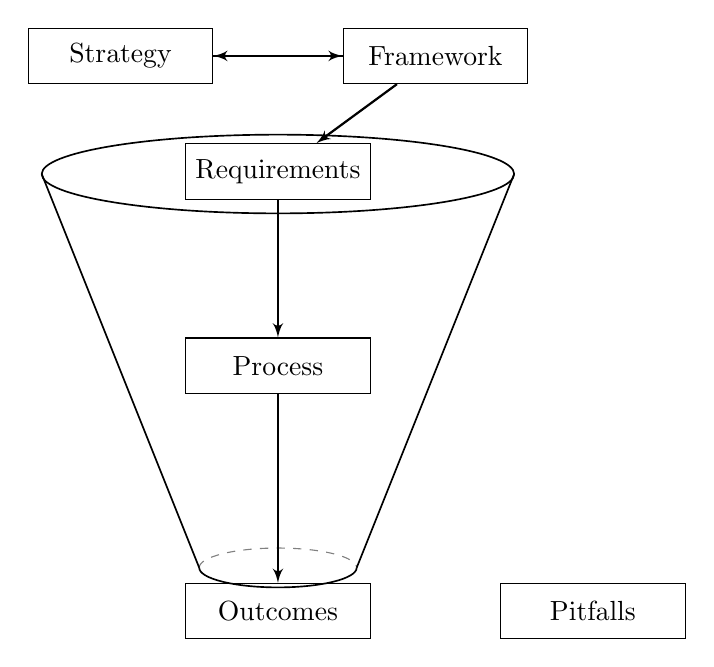
\begin{tikzpicture} [
   start chain=going below,    % General flow is top-to-bottom
    node distance=10mm and 40mm, % Global setup of box spacing
    ]
% ------------------------------------------------- 
\tikzset{
  base/.style={draw, on chain, on grid, align=center, minimum height=4ex},
  rect/.style={base, rectangle, minimum height=2em, text width=6em},
  line/.style={draw, thick, -latex'}
}

    \node [rect, xshift=-2.0cm, yshift=1.5cm] (stg) {Strategy};
    \node [rect, xshift=2.0cm, yshift=0.25cm] (req) {Requirements};
    \node [rect, yshift=-0.75cm] (prc) {Process};
    \node [rect, yshift=-1.4cm] (out) {Outcomes};
    \node [rect, right=of stg] (fmw) {Framework};
    \node [rect, right=of out] (pit) {Pitfalls};
    
    \draw[semithick] (-3,0) arc (180:0:3 and 0.5);                  % top ellipse top arc

    \draw[dashed,color=gray] (-1,-5) arc (180:0:1 and 0.25);        % bottom ellipse top arc
    \draw[semithick] (-1,-5) arc (-180:0:1 and 0.25);               % bottom ellipse bottom arc
    \draw[semithick] (-3,0) arc (-180:0:3 and 0.5);                 % top ellipse bottom arc
    \draw[semithick] (3,0) -- (1,-5);                               % funnel right side
    \draw[semithick] (-3,0) -- (-1,-5);                             % funnel left side
   
    \path [line] (stg) -- (fmw);
    \path [line] (fmw) -- (stg);
    \path [line] (fmw) -- (req);
    \path [line] (req) -- (prc);
    \path [line] (prc) -- (out); 

\end{tikzpicture}
\end{figure}

% Framework
% Integration and testing strategy
% Requirements for a framework - model-based testing, 
% Testing process - verification, the framework verifying non-functionalities
% Testing outcome
% Testing pitfalls
%%%%%%%%%%%%%%%%%%%%%%%%%%%%%%%%%%%%%%%%%%%%%%%%%%%%%%%%%%%%%%%%%%%%%%%%%%%
% Testing framework synthesis

% testing strategy
\section{Testing strategy}
Traditionally, testing is grouped to unit, integration, and system levels \citep{jenkins2008software}. Unit testing is assuring that individual software components and functions perform to specifications. When components are paired or grouped, the resulting connections must also be tested. Finally, system testing refers to testing the finished software suite with a suitable array of use cases.

The way integration testing is conducted is linked to the integration strategy. Service-
Oriented Architecture especially blurs the line between development and integration \citep{huang2008surrogate, wieczorek2010model}. \citet{myers1976software} introduces six integration strategies: bottom-up, top-down, modified top-down, sandwich, modified sandwich and big-bang testing. In the first two, integrations are put together and tested one by one, starting from either low-level systems or the most important system, whereas in big bang testing is delayed until the system is wholly integrated, where sandwich testing lies in between big-bang and top-down/bottom-up testing.

Other incremental testing methods include delivery, criticality, or functionality based 
strategies \citep{van2008identifying} where the system connections and hierarchy are built selectively an integration at a time. Further, \citet{carey1977control} discuss build testing. \citet{beizer1984software} introduces a "mixed bag" strategy which combines bottom-up, top-down, big-bang and build testing. 

% introduction of stubs and drivers
Delaying testing to the big-bang is not ideal for a large and complex integration undertaking because examining the integration as a whole and pinpointing defects is difficult. A better option might to test little by little and employ some other schemes. However, integration-by-integration testing requires drivers and stubs as stand-ins to make up for the absence of actual systems needed for tests.


Testing is an essential part of software engineering. Without a degree of confidence of sound operation and functional integrity, systems accumulate great risk and may ultimately produce more harm than benefit. Controlled testing reduces the number of incidents that would otherwise be discovered in the live environment and fixing which would be very expensive. In a similar fashion, testing can point to ways the systems can be improved. For example, a system that is fluid and easy to use does not incur as many service and maintenance or information requests. At the very least testing helps decision makers understand the risks involved in IT applications and services.

% TODO add references above chapters
Along with the functionality of the system, tests should also be applied on non-functional aspects such as performance and usability, because these also determine the validity of the system under test. Verifying that specified functions are implemented is not enough, but the system must satisfy underlying needs.

% What to test
Naturally, software has to be tested to after development, but there are other reasons, too. Any change in code or specifications, the environment, or testing policy or plans can act as a trigger for testing. Systematically repeating a set of tests to ascertain changes (like fixes) have not introduced new errors to previously functional code is called regression testing. The execution of regression tests is typically automated. A nearby concept, \textit{retesting} refers to examining if a fix has actually resolved an incident \citep{jenkins2008software}. Testing is a continous, and time-consuming, process.

% Out of scope?
\section{Integration testing pitfalls}

Testing management is no light matter: \citet{reid2005art} evaluated that about 50\% of system development time and more than 50\% of costs are spent on testing. Indeed, integration testing can fail in many ways \citep{van2008identifying}. Testing may be overlooked as a non-value adding activity and integration considered done as soon as systems have been connected. Alternatively, testing resources are considered expendable, and testing given a low priority, rendering it the project's 'crushable zone'. Not identifying and communicating integration strategy, responsibilities and accountabilities, lines of reporting and escalation -- or sharing knowledge -- are also typical pitfalls, according to \citet{van2008identifying}, exacerbated by lack of expertise and good document management. Additional problems are caused by physically separated locations, and failing configuration or incident management. \citep{van2008identifying}.

\citet{leung1990study} present a typology of integration errors and classify them to interpretation errors, interface errors and miscoded call errors, which are again divided into subgroups. The error types are presented in Figure X.

\begin{center}
    \begin{tabular}{ | l | p{3cm} | p{3cm} | p{3cm} |}
    \hline
    TODO & Interpretation error & Miscoded call error & Interface error \\ \hline
    Wrong & Unspecified function & Call at wrong location & Stardards or agreements are violated \\ \hline
    Missing & Not all necessary functionality implemented & Call instruction missing & Stardards or agreements are       violated \\ 
    \hline
    Extra & Function performs more than what is expected or needed & Call instruction on a path which should not have it & Stardards or agreements are violated \\
    \hline
    \end{tabular}
\end{center}

\begin{comment}
Interpretation
    wrong function - something else than specified
    extra function - more than what is expected/needed
    missing function - not all that is specified
Miscoded call (error which causes the developer to place the call instruction at the wrong point in the program)
    Extra instruction fault: the call instruction is on a path which should not have the call.
    Wrong placement fault: the call is at the wrong location on the path which should have the call instruction.
    Missing instruction fault: the call instruction is missing on the path which should have the call.
Interface error
    When stardards or agreements are violated
\end{comment}

% ERRORS: wrong function, extra function, missing function 
% Miscoded call error
% Interface error (Lueng \& white)

\section{Automation in testing}

Automating testing has obvious benefits of scale, but is not without fault. Implementing automated tests takes a significant initial investment of time and effort, algorithms cannot match the intelligence and intuition of an experienced human tester, while some systems undergo so many changes that automation makes little sense. As changes are introduced into the systems and code, related test cases must examined, their reusability ascertained, out-of-date cases should be discarded, and new cases created where necessary \citep{zhang2011approach}. Automation also does not counter inherently flawed software development processes. \citep{jenkins2008software, zhang2011approach).

Test case creation is perhaps the most time-consuming task in automated testing. Cases have to be produced based on the test plan and execution strategy, and updated when necessary. Researchers have presented solutions for automatic test case generation. \citet{tsai2002coyote} presents an XML-based framework for automated test case generation from WSDL service descriptions. \citet{bai2005WSDL} and \citet{di2007web} similarly offer WSDL service description based generation strategies. For regression testing, where the system suite is already in place, cases and related test data can be produced by recording actual use cases from production.

\section{Evaluating testing}

Before test cases are produced a strategy for their selection should be selected. Ideally the case set provides minimum required coverage based on the strategy criteria. \citet{benz2007combining} lists different schemes for testing strategy and case coverage based on e.g. traversal in the system network:
\begin{itemize}
\item Manual selection
\item Task coverage (each task performed once)
\item Simple Temporal Relationship Coverage (specified temporal relationships tested)
\item Complete Temporal Relationship Coverage (all temporal relationships tested)
\item n-Task combination coverage (each possible sequence of n-Tasks performed)
\item Interruption coverage (each possible interruption of task by other task tested)
\item Random selection of task sequences
\item Concurrency coverage
\item Pre- and post-condition based path coverages
\end{itemize}

\citet{linnenkugel1990test} present a similar coverage hierarchy of node, relation, call, sequence, and loop coverage measures.

\citet{bhuyan2012survey} present selection strategies for regression testing. Testing can be selective where only a part of the whole system is examined in order save time and costs. It is essential to model and understand the system hierarchy and which part of it should be tested. Code-based tests look for modified and related code that is tested, typically in unit tests. Testing can also be risk-based, recalling selective integration strategies. Risk areas are ones most affected by changes and which require the best coverage. In state-based regression testing coverage criteria are determined and test cases devised using control and data flow descriptions in UML state diagrams. Lastly, models, such as UML diagrams, can be used implemented regression testing for instance when access to code is not available. \citep{bhuyan2012survey}

The results of test effectiveness can be measured by how many cases were executed out of the set of necessary cases and testability by how many test cases are necessary for satisfying a criterion \citep{linnenkugel1990test}. Attention must be spent on both selecting the method of execution and test criteria. 

The test set quality itself can be evaluated quantitatively and 'tested'. In \citet{delmaro2011interface) mutation testing the test set quality is evaluated by creating variations of the tested programs and running the cases against the mutated programs. If it succeed against the mutated program, the case is considered live. Ideally, cases will fail when run against modified, erroneous code.

\section{Towards a model-based approach}
% add CIT definition earlier

Modeling is essential to understand and communicate system and component dependencies in 
integration and determining which connections are there to test. \citet{hewett2009automated} persuade testers to lay out and quantify components and their connections in a graph and use this information to design the 
most efficient order for testing, with a minimal need for creating test stubs. Likewise, \citet{leung1990study} and \citet{abdullah1995correcting} endorse the concept of a firewall, which draws a line between 
components and systems that are to be tested, and those that need not, based on where changes 
in code or specifications have occurred. Modeling can therefore point to systems that should 
be checked \textit{and} those that should be left out of testing scope (resembling Bhuyan's et al. selective testing). This both strengthens understanding of the inner workings of the tested system set-up and reduces testing costs. 
This kind of testing goes through the system(s) piece by piece while it disregards testing entire process chains.
 
In particular researchers advocate the creation of a call graph \citep{leung1990study, hurlburt2012not, linnenkugel1990test}, which explicitly maps interactions and relationships between integrated system components. The call graph can be used as a tool to communicate integration structures and schemes, and to organize testing. A systematic sweep of components and component connections is used to uncover any defects in the integration phase. 

The graph can serve as a foundation for setting test coverage criteria and strategy or test case creation 
\citep{benz2007combining, hura2011method, linnenkugel1990test}. Using model-driven integration \citet{wieczorek2010model} estimated savings of 50\% in time for test generation and concretization tasks.

\chapter{Piecing together a testing framework}
\label{chapter:framework}

\citet{huang2008surrogate} and \citet{liu2009unified} offer a unified testing framework for testing integration. The 
frameworks contain a generator for test cases, an execution engine, a surrogate engine 
simulating unavailable systems, and execution monitoring. Both frameworks are grounded on models or descriptions of the systems helping to automate stub or test case creation. Integration testing is done on a continuous basis (CIT, continuous integration testing) right from the start of development.

The figure below synthesizes integration testing theories and techniques introduced in the chapter. The model is based on the \citet{liu2009unified} unified testing framework model and adapted to Wärtsilä's integration testing needs. The model is technology-agnostic, and only presents the steps, systems, and processes required on an abstract level.

First off, production records are used for the genration of new test cases. This means that there must be some way to capture and record behaviour in the production environment, and save the information in a database. In the following generation step, the records are turned into an executable test case, which are then run by a testing engine agains the system under test (SUT). Models, diagrams, and specifications can also be used for automatically producing test cases. At least, models and specifications should be used to make sure the test cases address and measure correct things and defined behavior. The different types of records or models must be turned into cases in a way that the engine can run them. 

A surrogate engine refers to any scheme which is employed to act as a stand-in for unavailable, or testingwise unsuitable, systems. The surrogate engine's role is more important in the development phase, when not all components are fully ready.

As cases are run the execution traces or results are collected by . The traces are compared and verified with expected results determined by the test case and, if needed, also compared to execution engine records. 


\begin{figure}
\centering
% =================================================
\pgfdeclarelayer{marx}
\pgfsetlayers{main,marx}
\xdefinecolor{lightgrey}{RGB}{220,220,220}
\xdefinecolor{blackish}{RGB}{30,30,30}
% -------------------------------------------------
% Start the picture
\begin{tikzpicture}[
    start chain=going below,    % General flow is top-to-bottom
    node distance=6mm and 50mm, % Global setup of box spacing
    ]
% ------------------------------------------------- 
\tikzset{
  base/.style={draw, on chain, on grid, align=center, minimum height=4ex},
  proc/.style={base, rectangle, minimum height=4em, text width=7em},
  sut/.style={base, circle, text width=5em, fill = blackish, text = white},
  syst/.style={base, cylinder, shape border rotate=90,  aspect=.2, minimum height=5em, text width=5em},
  file/.style={base, rectangle, shape border rotate=90, minimum height=5em, text width=3em, fill = lightgrey},
  data/.style={base, trapezium, trapezium left angle=70, trapezium right angle=-70, minimum height=1cm}, 
  line/.style={draw, thick, -latex'}
}
% -------------------------------------------------
% Placing the nodes
\node [data] (s0) {Production};
\node [proc] (p0) {Integration test case generation};
\node [file] (f1) {Test case};
\node [syst] (e0) {Test case execution engine};
\node [sut] (s1) {SUT};
\node [syst] (e1) {Surrogate engine};
\node [file, right=of s0] (f0) {Model};
\node [proc, right=of f1] (p1) {Verification};
\node [file, right=of e0] (f2) {Exe-cution trace};
\node [proc, right=of s1] (p2) {Trace collecting};

\path [line] (s0) -- (p0);
\path [line] (p0) -- (f1);
\path [line] (f1) -- (e0);
\path [line] (e0) -- (s1);
\path [line] (s1) -- (e1);
\path [line] (f0) -- (p0);
\path [line] (f1) -- (p1);
\path [line] (p1) -- (e0);
\path [line] (s1) -- (p2);
\path [line] (p2) -- (f2);
\path [line] (f2) -- (p1);

\end{tikzpicture}
\caption{Testing framework hypothesis, adapted from \citet{liu2009unified}} \label{fig:UTF}
\end{figure}
% =================================================

% Thin threads, groupin into a tree (tsai et al)
% Test data difficult to select (linnenkugel mullburg)
% add background informtion: general about regression/integration/software testing, ITIL processes at Wärtsilä
% and possibly more...
% Todo: add Harness as testing strategy

\begin{comment}
% \input{2background.tex}
\chapter{Background}
\label{chapter:background}

The problem must have some background, otherwise it is not
interesting.  You can explain the background here. Probably you should
change the title to something that describes more the content of this
chapter. Background consists of information that help other masters of
the same degree program to understand the rest of the thesis.

Transitions mentioned in Section~\ref{section:structure} are used also
in the chapters and sections. For example, next in this chapter we
tell how to use English language, how to find and refer to sources,
and enlight different ways to include graphics in the thesis.

\section{Language and Structure}

Moreover, the transitions are also used in the paragraph and the
sentence level meaning that all the text is linked together. For example,
the word ``moreover'' here is one way, but of course you should use
variation in the text. Examples of transitional devices (words) and
their use can be found from writing guides, e.g. from the Online
Writing Lab
(OWL)\footnote{http://owl.english.purdue.edu/owl/resource/574/02/} of
Purdue University or Strunk's Elements of
Style\footnote{http://www.bartleby.com/141/}. Remember that footnotes
are additional information, and they are seldom used.  If you refer to a source, you do no
not use footnote. The right command for the references is \emph{cite}.

The language used in the thesis should be technical (or
scientifical). For example, the abreviations aren't used but all them
are written open (i.e. ``are not''). Since the content itself is often
hard to understand (and explain), the sentences should not be very
long, use complex language with several examples embedded in the same
sentence, and, also, seldom used words and weird euphemism or paraphrases
can make the sentence hard to follow and to read it with only one
time, and making everything even harder to understand all this without
any punctuation marks makes the instructor cry and finally after
trying to correct the language, you will get boomerang, and everyone's
time has just been wasted.

Please use proofreaders before sending even your unfinished version to
the instructor and/or supervisor. You will get better comments when
they do not need first proofread your text. Moreover, they can
consentrate to the content better if the language and spelling
mistakes are not distracting the reading. Several editors have their
own proofreading tools, e.g. ispell in emacs. You can also use
Microsoft Word to proofread your thesis: it can correct also some
grammatical errors and not just misspelled words.

Note also that if you have a section or a subsection, you have to have
at least two of them, or otherwise the section or subsection title is
unnecessary. Same with the paragraphs an: you should not have sections
with only one paragraphe, and single sentence paragraph. Furthermore,
always write some text after the title before the next level title.

\section{Finding and referring to sources}

Never ever copy anything into your theses from somebody else's text
(nor your own previously published text). Never. Not even for starting
point to be rewritten later. The risk is that you forgot the copied
text to your thesis and end up to be accused of plagiarism. Plagiarism
is a serious crime in studies and science and can ruin your career
even its beginning. To repeate: never cut and paste text into your
thesis!

\subsection{Finding sources}

All work is based on someone else's work. You should find the relevant
sources of your field and choose the best of them. Also, you should
refer to the original source where a fact has been mentioned first
time. Remember source evaluation (criticism) with all sources you
find.

Good starting points for finding references in computer science are:
\begin{itemize}
% You can use this command to set the items in the list closer to each other
% (ITEM SEParation, the vertical space between the list items)
\setlength{\itemsep}{0pt}
\item Nelli Portal (Aalto Library): \url{http://www.nelliportaali.fi}
\item ACM Digital library: \url{http://portal.acm.org/}
\item IEEExplore: \url{http://ieeexplore.ieee.org}
\item ScienceDirect: \url{http://www.sciencedirect.com/}
\item \ldots although Google Scholar (\url{http://scholar.google.com/}) will
find links to most of the articles from the abovementioned sources, if you
search from within the university network
\end{itemize}

Some of the publishers do not offer all the text of the articles
freely, but the library has agreed on the rights to use the whole
text. Thus, you should sometimes use computers in the domain of the
university in order to get the full text. Sometimes the Nelli Portal
can also help getting the whole article instead of just the abstract.
The library has also brief instrucions how to find
information~\cite{howfindinfo}.

Instead of normal Google, use Google Scholar
(\url{http://scholar.google.fi/}). It finds academic publications whereas
normal Google find too much commercial advertisements or otherwise
biased information. Wikipedia articles should be referred to in the master
thesis only very, very seldomly. You can use Wikipedia for understanding
some basics and finding more sources, but often you cannot be sure if
the article is correct and unbiased.

One important part of the sources that you have found is the reference
list. This way you can find the original sources that all the other
research of the field refer. Often you can also find more information
with the name of the researchers that are often referred in the
articles.

\subsection{Referring to sources}

The main point in referring to sources is to separate your own
thinking and text from that of others. Facts of the research area can
be given without reference, but otherwise you should refer to
sources. This means two things: marking the source in the text where
it has been used, and listing the sources usually in the end of the
thesis in a way that help the reader to find the original source.

There are several bibliography styles, meaning how to form the
bibliography in the end of the thesis. Aalto's library has good
instructions for many styles~\cite{bibinstructions}. You should ask
from your supervisor or instructors which style you should use. This
thesis template uses the number style that is often used in software
engineering. The other style also used in the CS field,
e.g. usability, is the Harvard style where instead of numbers, the
reference is marked into the text with author's name and publishing
year. Other areas use also many other styles for making the lists and
marking the references.

In addition to the list in the end of the thesis, you have to mark the
source in the text where the source is used. There are three places
for the reference: in a sentence before the period, in the end of a
sentence after the period, or in the end of a paragraph. All of them
have different meaning. The main point is that first you paraphrase
the source using your own words and then mark the source. Next, we
give short examples that are marked with \emph{emphasised text}.

\emph{Haapasalo~\cite{HaapasaloThesis} researched database algorithms
  that allows use of previous versions of the content stored in the
  database.} This kind of marking means that this paragraph (or until
the next reference is given) is based on the source mentioned in the
beginning.  Giving the source you should use only the family name of
the first author of the article, and not give any hints about what is
the type of the article that is referred.

\emph{B+-trees offers one way to index data that is stored in to a
  database. Multiversion B+-trees (MVBT) offer also a way to restore
  the data from previous versions of the database. Concurrent MVBT
  allows many simultaneous updates to the database that is was not
  possible with MVBT.~\cite{HaapasaloThesis}} When the marking is
after the period, the reference is retrospective: all the paragraph
(or after previous reference marking) is based on the source given in
its end. If the content is very broad, you can start with saying
\emph{According to Haapasalo}, then continue referring the source with
several separate sentences, and in the end put the marking of your
source \emph{ that shows that CMVBT are the
  best. ~\cite{HaapasaloThesis}}.

If your paragraph has several sources, the above mentioned styles are
not proper. The reader of your thesis cannot know which of your
sources give which of the statements. In this case, it is better to
use more finegraded refering where the reference markings that are
embedded in the sentences. For example, \emph{the multiversion B+-tree
  (MVBT) index of Becker et al.~\cite{becker:1996:mvbt} allows database
  users to query old versions of the database, but the index is not
  transactional.
  It's successor, the transactional MBVT (TMVBT), allows a single transaction
  running in its own thread or process to update the database concurrently
  with other transactions that only read the
  database~\cite{haapasalo:2009:tmvbt}.
  Further development, titled the concurrent MBVT (CMVBT),
  allows several transactions to perform updates to the database at the same
  time~\cite{HaapasaloThesis}}.
  Here, the references are marked before
  the period in the sentences where they are used.

Finally, direct quotes are allowed. However, often you should avoid
them since they do not usually fit in to your text very well. Using
direct quotes has two tricks: quotation marks and the source.  \emph{
  ``Even though deletions in a multiversion index must not physically
  delete the history of the data items, queries and range scans can
  become more efficient, if the leaf pages of the index structure are
  merged to retain optimality.''~\cite{HaapasaloThesis}} Quotes are
hard to make neatly since you should use only as much as needed
without changing the text. Moreover, you often do not really
understand what the author has mentioned with his wordings if you
cannot write the same with your own words. Remember also that never
cut and paste anything without marking the quotation marks right away,
and in general, never cut and paste anything at all!

Sometimes getting the original source can be almost impossible. In an
extremely desperate situation, you can refer with structure \emph{mr
  X~[\ldots] according to ms Y~[\ldots] defined that}, if you find a
source that refers to the original source. Note also that the
reference marking is never used as sentence element (example of how
\textbf{not} to do it: \emph{\cite{HaapasaloThesis} describes
an optimal algorithm for indexing multiversiond databases.}).



% \input{3environment.tex}

\chapter{Environment}
\label{chapter:environment}

A problem instance is rarely totally independent of its environment.
Most often you need to describe the environment you work in, what
limits there are and so on. This is a good place to do that. First we
tell you about the LaTeX working environments and then is an example
from an thesis written some years ago.


\section{LaTeX working environments}
\label{sec:environments}

To create \LaTeX\ documents you need two things: a \LaTeX\ environment for
compiling your documents and a text editor for writing them.

\subsection{Environment}

Fortunately \LaTeX\ can nowadays be found for any (modern) computer
environment, be it Linux, Windows, or Macintosh.
For Linuxes (and other Unix clones) and Macs, I'd recommend \emph{TeX
Live}~\cite{TeXLive}, which is the current default \LaTeX\ distribution for
many Linux flavors such as Fedora, Debian, Ubuntu, and Gentoo.
TeX Live is the replacement for the older \emph{teTeX}, which is
no longer developed.

TeX Live works also for Windows machines (at least according to their web
site); however, I have used \emph{MiKTeX}~\cite{MiKTeX} and can recommend it
for Windows.
MiKTeX has a nice package manager and automatically fetches missing packages
for you.

\subsection{Editor}

You can write \LaTeX\ documents with any text editor you like, but having
syntax coloring options and such really helps a lot.
My personal favourite for editing \LaTeX\ is the
\emph{TeXlipse}~\cite{TeXlipse} plugin for the Eclipse IDE~\cite{Eclipse}.
Eclipse is an open-source integrated development environment (IDE) initially
created for writing Java code, but it currently has support for editing
languages such as C, C++, JavaScript, XML, HTML, and many more.
The TeXlipse plugin allows you to edit and compile \LaTeX\ documents directly
in Eclipse, and compilation errors and warnings are shown in the Eclipse
\emph{Problems} dialog so that you can locate and fix the issues easily.
The plugin also supports reference traversal so that you can locate the source
line where a label or a citation is defined.

Eclipse is an entire development environment, so it may feel a bit heavy-weight
for editing a document.
If you are looking for a more light-weight option, check out TeXworks.
TeXworks is a \LaTeX\ editor that is packaged with the newer MiKTeX
distributions, and it can be acquired from \url{http://www.tug.org/texworks/}.

And if you are attached to your \emph{emacs} or \emph{vim} editor, you
can of course edit your \LaTeX\ documents with them.
Emacs at least has syntax coloring and you can compile your document with a key
binding, so this may be a good option if you prefer working with the standard
Linux text editors.

\section{Graphics}

When you use \texttt{pdflatex} to render your thesis, you can include PDF images
directly, as shown by Figure~\ref{fig:indica_model} below.

\begin{figure}[ht]
  \begin{center}
    \includegraphics[width=\textwidth]{example_indica_model.pdf}
    \caption{The INDICA two-layered value chain model.}
    \label{fig:indica_model}
  \end{center}
\end{figure}

You can also include JPEG or PNG files, as shown by Figure~\ref{fig:eeyore}.

\begin{figure}[ht]
  \begin{center}
    \includegraphics[width=9cm]{example_ihaa.jpg}
    \caption{Eeyore, or Ihaa, a very sad donkey.}
    \label{fig:eeyore}
  \end{center}
\end{figure}

You can create PDF files out of practically anything.
In Windows, you can download PrimoPDF or CutePDF (or some such) and install a
printing driver so that you can print directly to PDF files from any
application. There are also tools that allow you to upload documents in common
file formats and convert them to the PDF format.
If you have PS or EPS files, you can use the tools \texttt{ps2pdf} or
\texttt{epspdf} to convert your PS and EPS files to PDF\@.

% Comment: If your sentence ends in a capital letter, like here, you should
% write \@ before the period; otherwise LaTeX will assume that this is not
% really an end of the sentence and will not put a large enough space after the
% period. That is, LaTeX assumes that you are (for example), enumerating using
% capital roman numerals, like I. do something, II. do something else. In this
% case, the periods do not end the sentence.

% Similarly, if you do need a normal space after a period (instead of
% the longer sentence separator), use \  (backslash and space) after the
% period. Like so: a.\ first item, b.\ second item.

Furthermore, most newer editor programs allow you to save directly to the PDF
format. For vector editing, you could try Inkscape, which is a new open source
WYSIWYG vector editor that allows you to save directly to PDF\@.
For graphs, either export/print your graphs from OpenOffice Calc/Microsoft
Excel to PDF format, and then add them; or use \texttt{gnuplot}, which can
create PDF files directly (at least the new versions can).
The terminal type is \emph{pdf}, so the first line of your plot file should be
something like \texttt{set term pdf \ldots}.

To get the most professional-looking graphics, you can encode them using the
TikZ package (TikZ is a frontend for the PGF graphics formatting system).
You can create practically any kind of technical images with TikZ, but it has a
rather steep learning curve. Locate the manual (\texttt{pgfmanual.pdf}) from
your \LaTeX\ distribution and check it out. An example of TikZ-generated
graphics is shown in Figure~\ref{fig:page-merge}.

\begin{figure}[ht]
  \begin{center}
    \input{example_page-merge.tex}
    \caption{Example of a multiversion database page merge. This figure has
    been taken from the PhD thesis of Haapasalo~\cite{HaapasaloThesis}.}
    \label{fig:page-merge}
  \end{center}
\end{figure}

Another example of graphics created with TikZ is shown in
Figure~\ref{fig:tikz-examples}.
These show how graphs can be drawn and labeled.
You can consult the example images and the PGF manual for more examples of what
kinds figures you can draw with TikZ.

% These definitions are only used in the example images; you will not
% need them for your thesis...
\newlength{\graphdotsize}
\setlength{\graphdotsize}{1.7pt}
\newlength{\graphgridsize}
\setlength{\graphgridsize}{1.2em}
\begin{figure}[ht]
\begin{center}
\subfigure[Examples of obstruction graphs for the Ferry Problem]{
  \input{example_obstruction-grouped.tex}
}
\subfigure[Examples of star graphs]{
  \input{example_general-star-graphs.tex}
}
\caption{Examples of graphs draw with TikZ. These figures have been taken from a
course report for the graph theory course~\cite{FerryProblem}.}
\label{fig:tikz-examples}
\end{center}
\end{figure}

% \input{4methods.tex}

\chapter{Methods}
\label{chapter:methods}

You have now stated your problem, and you are ready to do something
about it!  \emph{How} are you going to do that? What methods do you
use?  You also need to review existing literature to justify your
choices, meaning that why you have chosen the method to be applied in
your work.

% An example of a traditional LaTeX table
% ------------------------------------------------------------------
% A note on underfull/overfull table cells and tables:
% ------------------------------------------------------------------
% In professional typography, the width of the text in a page is always a lot
% less than the width of the page. If you are accustomed to the (too wide) text
% areas used in Microsoft Word's standard documents, the width of the text in
% this thesis layout may suprise you. However, text in a book needs wide
% margins. Narrow text is easier to read and looks nicer. Longer lines are
% hard to read, because the start of the next line is harder to locate when
% moving from line to the next.
% However, tables that are in the middle of the text often would require a wider
% area. By default, LaTeX will complain if you create too wide tables with
% ``overfull'' error messages, and the table will not be positioned properly
% (not centered). If at all possible, try to make the table narrow enough so
% that it fits to the same space as the text (total width = \textwidth).
% If you do need more space, you can either
% 1) ignore the LaTeX warnings
% 2) use the textpos-package to manually position the table (read the package
%    documentation)
% 3) if you have the table as a PDF document (of correct size, A4), you can use
%    the pdfpages package to include the page. This overrides the margin
%    settings for this page and LaTeX will not complain.
% ------------------------------------------------------------------
% Another note:
% ------------------------------------------------------------------
% If your table fits to \textwidth, but the cells are so narrow that the text
% in p{..}-formatted cells does not flow nicely (you get underfull warnings
% because LaTeX tries to justify the text in the cells) you can manually set
% the text to unjustified by using the \raggedright command for each cell
% that you do not want to be justified (see the example below). \raggedleft
% is also possible, of course...
% ------------------------------------------------------------------
% If you need to have linefeeds (\\) inside a cell, you must create a new
% paragraph-formatting environment inside the cell. Most common ones are
% the minipage-environment and the \parbox command (see LaTeX documentation
% for details; or just google for ``LaTeX minipage'' and ``LaTeX parbox'').
\begin{table}
\begin{tabular}{|p{2cm}|p{3.8cm}|p{4.5cm}|p{1.1cm}|}
% Alignment of sells: l=left, c=center, r=right.
% If you want wrapping lines, use p{width} exact cell widths.
% If you want vertical lines between columns, write | above between the letters
% Horizontal lines are generated with the \hline command:
\hline % The line on top of the table
\textbf{Code} & \textbf{Name} & \textbf{Methods} & \textbf{Area} \\
\hline
% Place a & between the columns
% In the end of the line, use two backslashes \\ to break the line,
% then place a \hline to make a horizontal line below the row
T-110.6130 & Systems Engineering for Data Communications
    Software & \raggedright Computer simulations, mathematical modeling,
  experimental research, data analysis, and network service business
  research methods, (agile method) & T-110 \\
\hline
\multicolumn{2}{|p{6.25cm}|}{Mat-2.3170 Simulation (here is an example of
 multicolumn for tables)}& Details of how to build simulations & T-110 \\
% The multicolumn command takes the following 3 arguments:
% the number of cells to merge, the cell formatting for the new cell, and the
% contents of the cell
\hline
S-38.3184 & Network Traffic Measurements and Analysis
& \raggedright How to measure and analyse network
  traffic & T-110 \\ \hline
\end{tabular} % for really simple tables, you can just use tabular
% You can place the caption either below (like here) or above the table
\caption{Research methodology courses}
% Place the label just after the caption to make the link work
\label{table:courses}
\end{table} % table makes a floating object with a title

If you have not yet done any (real) metholodogical courses (but chosen
introduction courses of different areas that are listed in the
methodological courses list), now is the time to do so or at least
check through material of suitable methodological courses. Good
methodologial courses that consentrates especially to methods are
presented in Table~\ref{table:courses}. Remember to explain the
content of the tables (as with figures). In the table, the last column
gives the research area where the methods are often used. Here we used
table to give an example of tables. Abbreviations and Acronyms is also
a long table. The difference is that longtables can continue to next
page.

% \input{5implementation.tex}

\chapter{Implementation}
\label{chapter:implementation}

You have now explained how you are going to tackle your problem.
Go do that now! Come back when the problem is solved!

Now, how did you solve the problem?
Explain how you implemented your solution, be it a software component, a
custom-made FPGA, a fried jelly bean, or whatever.
Describe the problems you encountered with your implementation work.

% \input{6evaluation.tex}

\chapter{Evaluation}
\label{chapter:evaluation}

You have done your work, but that's\footnote{By the way, do \emph{not} use
shorthands like this in your text! It is not professional! Always write out all
the words: ``that is''.} not enough.

You also need to evaluate how well your implementation works.  The
nature of the evaluation depends on your problem, your method, and
your implementation that are all described in the thesis before this
chapter.  If you have created a program for exact-text matching, then
you measure how long it takes for your implementation to search for
different patterns, and compare it against the implementation that was
used before.  If you have designed a process for managing software
projects, you perhaps interview people working with a waterfall-style
management process, have them adapt your management process, and
interview them again after they have worked with your process for some
time. See what's changed.

The important thing is that you can evaluate your success somehow.
Remember that you do not have to succeed in making something spectacular; a
total implementation failure may still give grounds for a very good master's
thesis---if you can analyze what went wrong and what should have been done.


% \input{7discussion.tex}

\chapter{Discussion}
\label{chapter:discussion}

At this point, you will have some insightful thoughts on your implementation
and you may have ideas on what could be done in the future.
This chapter is a good place to discuss your thesis as a whole and to show your
professor that you have really understood some non-trivial aspects of the
methods you used\ldots


% \input{8conclusions.tex}

\chapter{Conclusions}
\label{chapter:conclusions}

Time to wrap it up!
Write down the most important findings from your work.
Like the introduction, this chapter is not very long.
Two to four pages might be a good limit.
\end{comment}


% Load the bibliographic references
% ------------------------------------------------------------------
% You can use several .bib files:
% \bibliography{thesis_sources,ietf_sources}
\bibliography{ref}


% Appendices go here
% ------------------------------------------------------------------
% If you do not have appendices, comment out the following lines
\appendix
% \input{appendices.tex}

\chapter{First appendix}
\label{chapter:first-appendix}

This is the first appendix. You could put some test images or verbose data in an
appendix, if there is too much data to fit in the actual text nicely.

For now, the Aalto logo variants are shown in Figure~\ref{fig:aaltologo}.

\begin{figure}
\begin{center}
\subfigure[In English]{\includegraphics[width=.8\textwidth]{aalto-logo-en}}
\subfigure[Suomeksi]{\includegraphics[width=.8\textwidth]{aalto-logo-fi}}
\subfigure[Pä svenska]{\includegraphics[width=.8\textwidth]{aalto-logo-se}}
\caption{Aalto logo variants}
\label{fig:aaltologo}
\end{center}
\end{figure}


% End of document!
% ------------------------------------------------------------------
% The LastPage package automatically places a label on the last page.
% That works better than placing a label here manually, because the
% label might not go to the actual last page, if LaTeX needs to place
% floats (that is, figures, tables, and such) to the end of the
% document.
\end{document}